\chapter{Bedienungs-Anleitung}

\section{Installation}

Android-Applikationen werden in einem speziellen Paket-Format mit der Datei-Endung ``.apk'' ausgeliefert. Normalerweise würde ein Benutzer dieses von dem von Google betriebenen Applikations-Katalog \emph{Android Market} herunterladen und installieren. Da die Auslieferung an Endbenutzer nicht in den Umfang dieser Arbeit fällt, wurde die entwickelte Applikation nicht in diesem veröffentlicht und muss manuell vom Benutzer auf das Endgerät kopiert und dort installiert werden.

Ist das Android Software Development Kit (SDK) verfügbar, kann die Applikation über die in Eclipse integrierte Entwicklungsumgebung namens ``Android Development Tools'' (ADT) installiert werden. Das Kommandozeilen-Programm ``adb'' (Android Developer Bridge) dient dabei als Brücke zum jeweiligen Gerät (oder dem Emulator). Mit dem Install-Kommando kann damit eine Applikation installiert werden.

\begin{lstlisting} [caption={Installation der Applikation},label=adb_install]
> $SDK_DIR/tools/adb install <applikation.apk>
\end{lstlisting}

Nach der Installation muss die Eingabe-Methode noch aktiviert werden. Dies geschieht im den globalen Einstellungen von Android. Diese werden vom Home-Screen aus mit dem Menü-Punkt ``Einstellungen'', unter ``Sprache  \& Tastatur''. Hier muss der entsprechende Menü-Punkt für unsere Eingabe-Methode namens ``HandwritingIME'' aktiviert werden, worauf der Benutzter vor den möglichen Risiken einer Eingabe-Methode eines Drittanbieters hingewiesen wird.

\begin{figure}[h!]
   \centering
   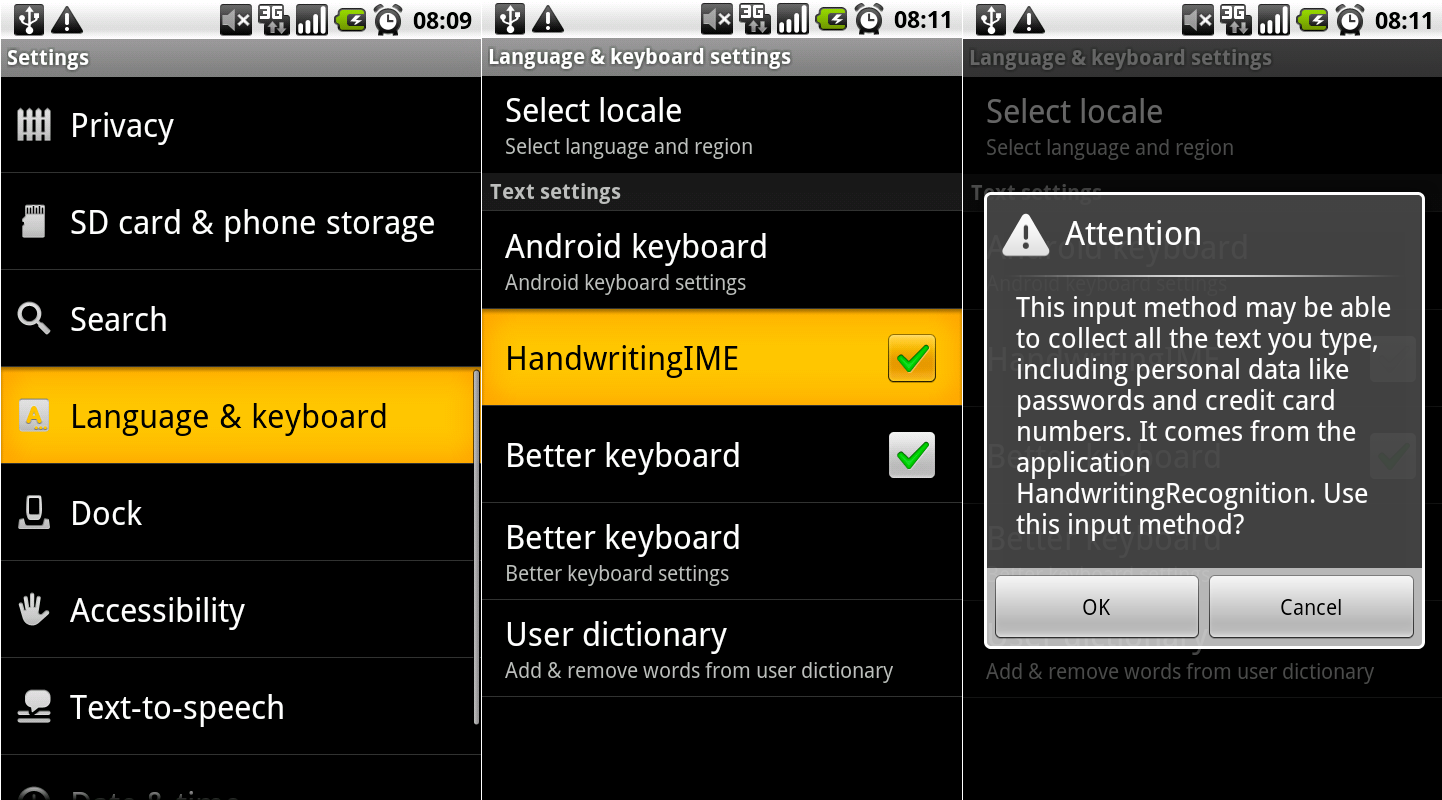
\includegraphics[scale=0.15]{img/manual_activate} 
   \caption{Aktivierung der Eingabe-Methode}
   \label{fig:manual_activate}
\end{figure}

Nun muss die Eingabe-Methode noch als der systemweite Standard festgelegt werden. Dazu muss das so genannte ``Long-Press''-Menü eines beliebigen Textfeldes aufgerufen werden. Dies geschieht, indem für etwa 1-2 Sekunden auf das Eingabefeld gedrückt wird, worauf das Menü angezeigt wird. Nun muss unter dem Menü-Punkt ``Eingabemethode'' unsere Methode angewählt werden. Falls nötig, erfolgt das Zurücksetzen auf die mitgelieferte Eingabe-Methode über den selben Weg, nur das jetzt die entsprechende Methode ausgewählt wird.

\begin{figure}[h!]
   \centering
   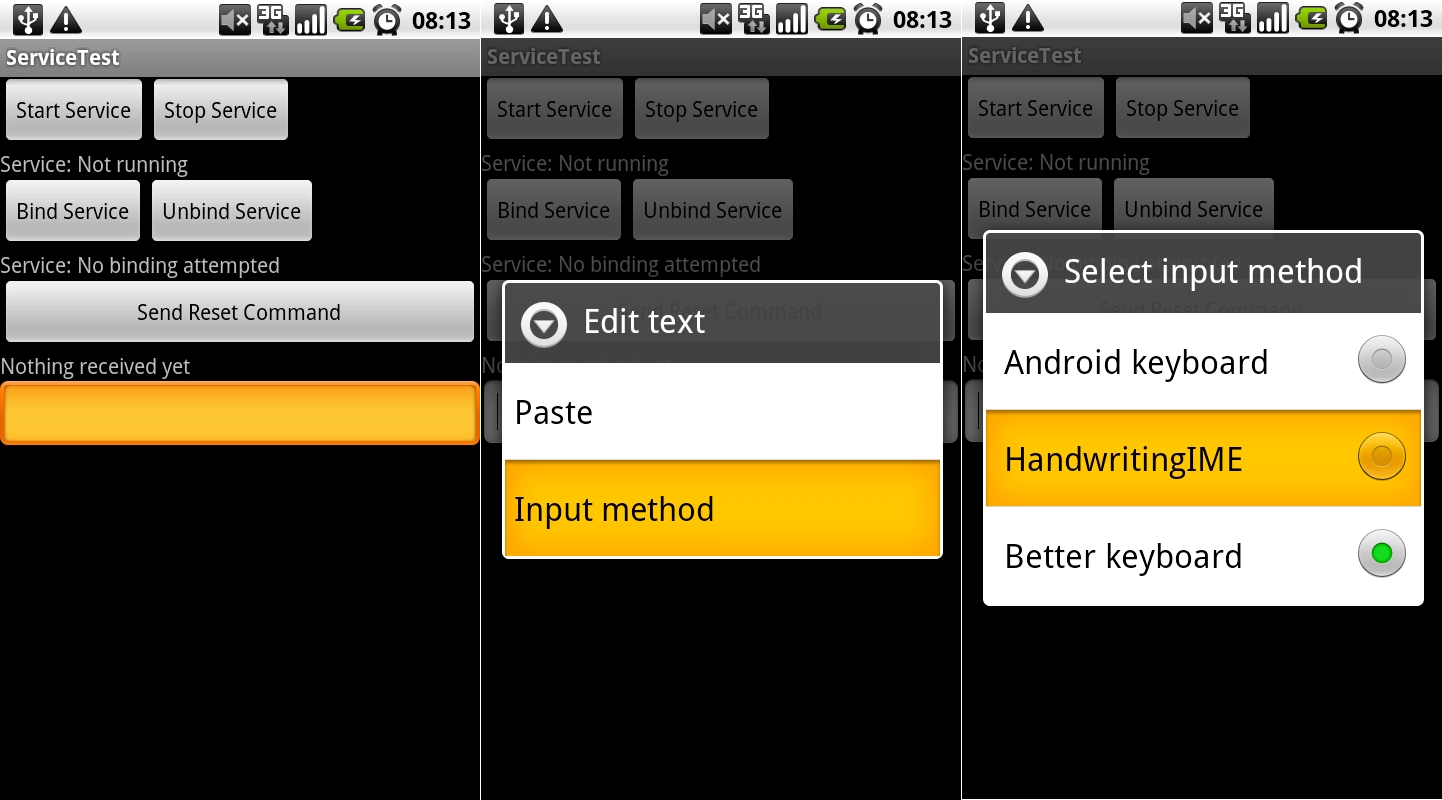
\includegraphics[scale=0.15]{img/manual_ime_select} 
   \caption{Auswählen der Eingabe-Methode}
   \label{fig:manual_ime_select}
\end{figure}

Nun wird beim Auswählen eines Eingabefeldes unsere Eingabe-Methode angezeigt. Beim ersten Aufrufen kann es zu einer kurzen Verzögerung kommen, da der Erkennungs-Dienst ebenfalls initialisiert werden muss. Weiter Aufrufe sollten unverzüglich erfolgen.

\section{Bedienung}

\begin{figure}[h!]
   \centering
   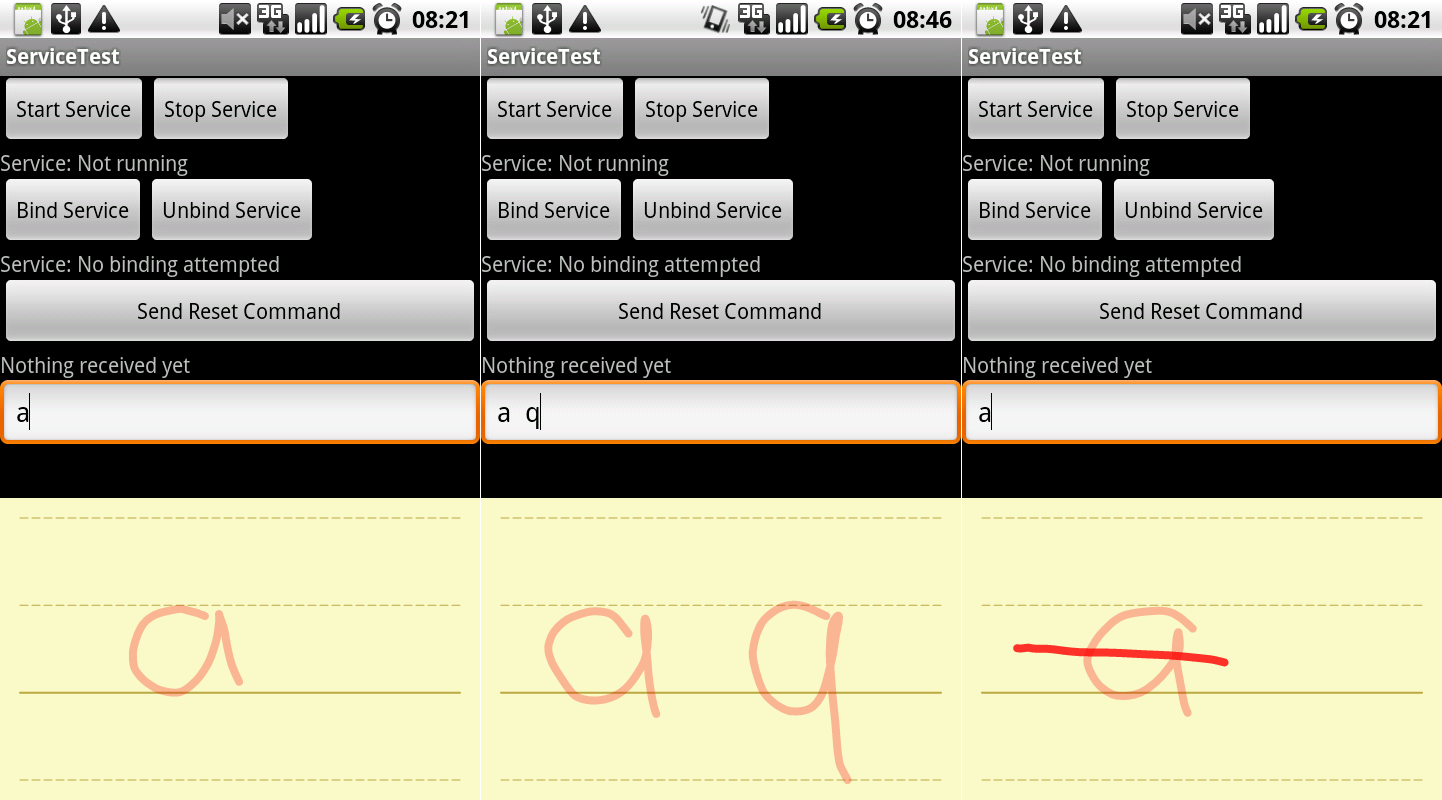
\includegraphics[width=\textwidth]{img/manual_input} 
   \caption{Verwendung der Eingabe-Methode}
   \label{fig:manul_input}
\end{figure}

Damit ist die Eingabe von Zeichen in Handschrift möglich. Wurde ein Zeichen falsch erkannt, kann das jeweils letztmalig eingegebene Zeichen gelöscht werden, indem es von vollständig von links nach rechts durchgestrichen wird. Wird zwischen einer neuen Eingabe und dem letzten eingegebenen Zeichen ein Abstand von mindestens der Breite des letzten Zeichens eingehalten, wird automatisch ein Leerzeichen eingefügt.

\begin{figure}[h!]
   \centering
   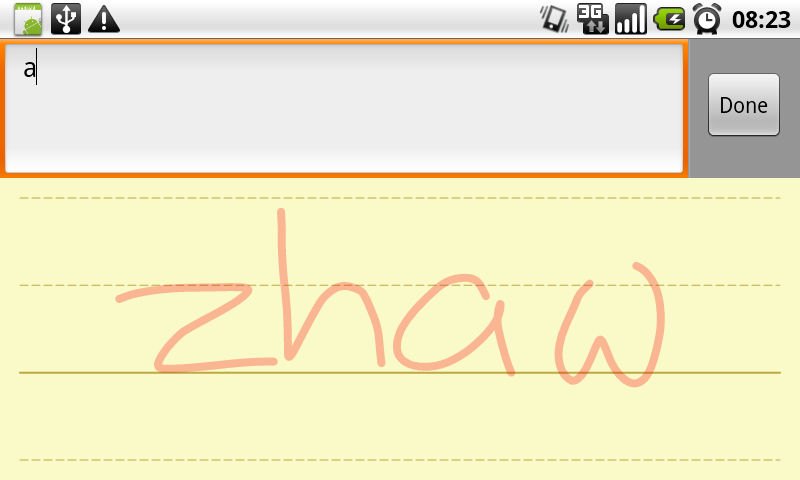
\includegraphics[width=\textwidth]{img/manual_landscape} 
   \caption{Verwendung der Eingabe-Methode im Querformat}
   \label{fig:manual_landscape}
\end{figure}

Um die Eingabe-Methode wieder zu verlassen wird die Zurück-Taste des Endgeräts verwendet.

